\documentclass[a4paper]{article}
\usepackage[utf8]{inputenc}

\usepackage{acronym}
\usepackage{amsmath}
\usepackage[USenglish]{babel}
\usepackage[style=ieee]{biblatex}
\usepackage{color}
\usepackage[a4paper]{geometry}
\usepackage{graphicx}
\usepackage{hyperref}
\usepackage{listings}
\usepackage{listings-rust/listings-rust}
% No indent after paragraphs
\usepackage{parskip}
\usepackage{siunitx}

% Define paper size
\geometry{outer=2.5cm, inner=2.5cm, top=3.5cm, bottom=3.5cm}

% Configure lstlistings
\definecolor{beige}{RGB}{255, 245, 240}
\lstset{
    backgroundcolor=\color{beige},
    frame=single,
    keepspaces=true,
    captionpos=b,
    breaklines=true,
}

\addbibresource{references.bib}

\title{Agent-Based Models in Cellular Systems}

\begin{document}
% TITLEPAGE

\maketitle

\pagebreak
\tableofcontents

%###################################################################################################
\begin{abstract}
\end{abstract}

%###################################################################################################
\section{Introduction}
\subsection{Individual-Based Nature of Biology}
\subsection{Mathematical and Numerical Treatment}
\subsection{Questions that can be answered with this approach}

%###################################################################################################
\section{ABM Theory}
\subsection{Theoretical Framework}
\subsection{Parameter Estimation \& Sensitivity Analysis}
\subsection{Coarse-Graining}
\subsection{Pattern Formation}

%###################################################################################################
\pagebreak
\section{cellular\_raza: A novel Agent-Based Framework}
\cite{Pleyer2025}
\subsection{Goals}
\subsection{Structure \& Development}
\subsection{Functionality \& Limitations}

\subsection{Benchmarks}
This section provides multiple benchmarks which can be read and unserstood separately.
Their purpose is to provide insights into performance characteristics and assert the correctness of
the solvers and routines used within \texttt{cellular\_raza}.

\subsubsection{Multithreading Performance (Amdahl's Law)}

\paragraph{Theory}
One measure of multithreaded performance is to calculate the possible theoretical speedup
given by Amdahl's law~\cite{Rodgers1985}.
It provides an estimate for the speedup and assumes that the workload can be split into a
parallelizable and non-parallelizable part which is quantified by $0\leq p \leq1$.
A higher value means that the contribution coming from non-parallelizable algorithms is lower.
The theoretical maximum $p=1$ means that all of the executed code is parallelizable.
Amdahl's law is given by

\begin{equation}
    T(n) = T_0\frac{1}{(1-p) + \frac{p}{n}}
    \label{eq:amdahls-law}
\end{equation}

where $T(n)$ describes the throughput which can be achieved given $n$ parallel threads and the
variable $p$ is the relative proportion of execution time which benefits from parallelization.
The total latency of a program can be determined via the inverse of the throughput.

\paragraph{Simulation Setup}
Measuring the performance of any simulation will be highly dependent on the specific cellular 
properties and complexity.
For this comparison, we chose the previously explained cell-sorting example which contains minimal
complexity compared to other examples (see
\href{https://cellular-raza.com/showcase}{cellular-raza.com/showcase}).
Any computational overhead which is intrinsic to \texttt{cellular\_raza} and not related to the
chosen example would thus be more likely to manifest itself in performance results.

In order to produce reproducible results and simplify this overall process, we provide the
\href{https://github.com/jonaspleyer/cellular_raza/tree/master/cellular_raza-benchmarks}{cellular\_raza-benchmarks} crate.
It is a command-line utility which can be used to run benchmarks with various configurations.
Its arguments are displayed in Listing~\ref{listing:benchmarks-cli}.

\begin{minipage}{\linewidth}\begin{lstlisting}[
    language=Bash,
    basicstyle=\ttfamily\footnotesize,
    label=listing:benchmarks-cli,
    caption={
        Usage of the benchmark CLI tool.
        We provide two benchmarks, one for increasing the number of agents and another for
        increasing the number of threads.
        The subcommands can be further customized and will automatically run the given simulation
        multiple times for the specified configurations.
    }
]
Usage: cell_sorting [OPTIONS] <NAME> [COMMAND]

Commands:
  threads   Thread scaling benchmark
  sim-size  Simulation Size scaling benchmark
  help      Print this message or the help of the given subcommand(s)

Arguments:
  <NAME>  Name of the current runs such as name of the device to be benchmarked

Options:
  -o, --output-directory <OUTPUT_DIRECTORY>
          Output directory of benchmark results [default: benchmark_results]
  -s, --sample-size <SAMPLE_SIZE>
          Number of samples to be generated for each measurement [default: 5]
      --no-save
          Do not save results. This takes priority against the overwrite settings
      --overwrite
          Overwrite existing results
      --no-output
          Disables output
  -h, --help
          Print help
  -V, --version
          Print version
\end{lstlisting}\end{minipage}

Results generated in this way are stored inside the \texttt{benchmark\_results} folder.
In addition, we provide a python script \texttt{plotting/cell\_sorting.py} to quickly visualize
the obtained results.

\paragraph{Hardware}
We ran this benchmark on three distinct hardware configurations.
Although there exists a wide range of variables which could influence our measured runtime results,
we expect that the biggest effects are due to power-limits and variable frequency of the
central processing unit (CPU) (see Figure~\ref{tab:hardware-configurations}).
Both of these effects can be circumvented by choosing an artificially fixed frequency which is low
enough such that the total power limit of the CPU is never reached even when multiple cores are
under load.
While it is well known that other aspects such as cache-size and memory latency can have an impact
on absolute performance, they should however not introduce any significant deviations in terms of
relative performance scaling.

\begin{table}
    \centering
    \begin{tabular}{l c c c}
        CPU & Fixed Clockspeed & Memory Frequency & TDP\\
        \hline
        AMD Ryzen 3700X~\cite{AMDProductSpecifications} & $\SI{2200}{\mega\hertz}$
            & $\SI{3200}{\mega T\per\second}$ & $\SI{65}{\watt}$\\
        AMD Ryzen Threadripper 3960X~\cite{AMDProductSpecifications} & $\SI{2000}{\mega\hertz}$
            & $\SI{3200}{\mega T\per\second}$ & $\SI{280}{\watt}$\\
        Intel Core i7-12700H~\cite{Inteli712700H} & $\SI{2000}{\mega\hertz}$
            & $\SI{4800}{\mega T\per\second}$
            & $\SI{45}{\watt}$\\
    \end{tabular}
    \caption{List of tested hardware configurations.}
    \label{tab:hardware-configurations}
\end{table}

\paragraph{Results}

\begin{figure}
    \centering
    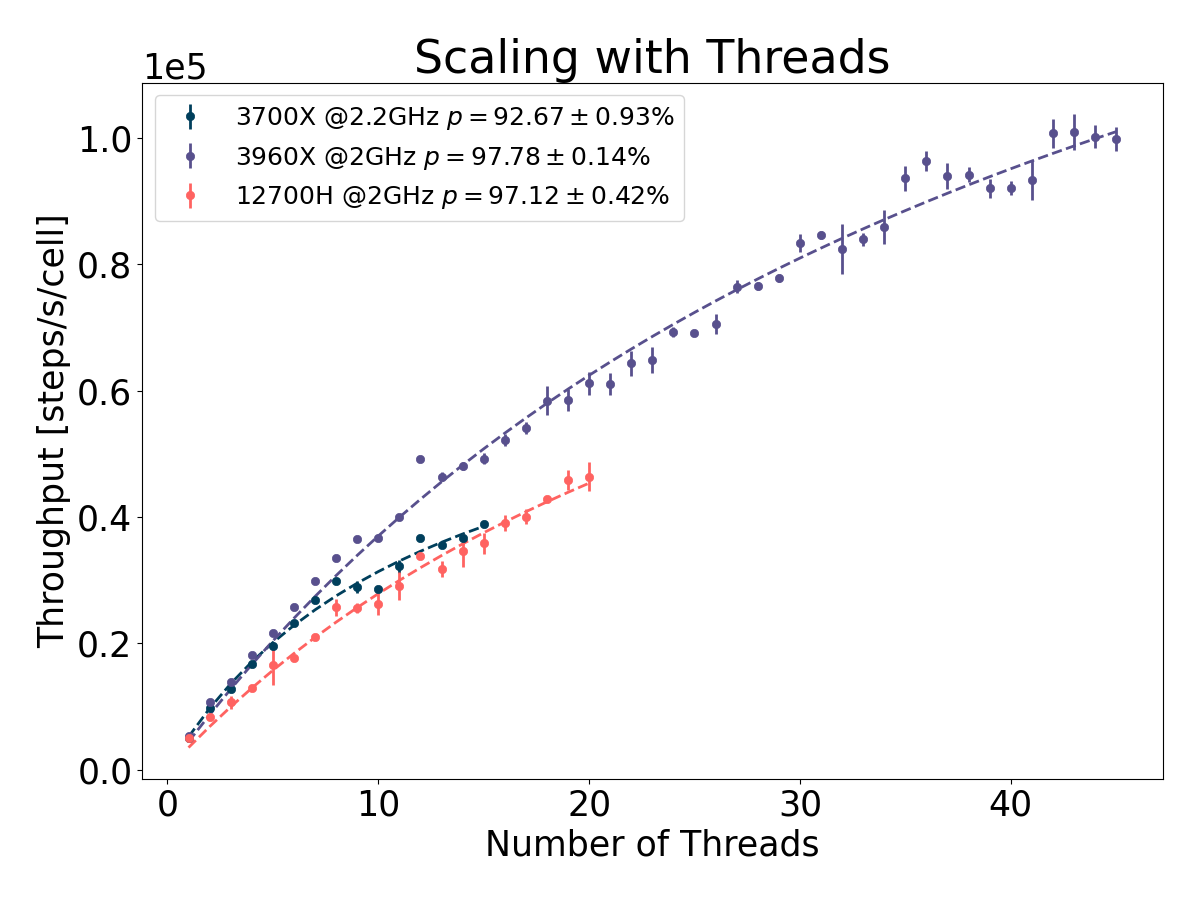
\includegraphics[width=0.8\textwidth]{cellular_raza-homepage/static/benchmarks/thread_scaling.png}
    \caption{Performance of the throughput $T(n)$ for increasing number of utilized threads $n$.}
    \label{fig:amdahls-law-fit}
\end{figure}

In figure~\ref{fig:amdahls-law-fit}, we fit Amdahl's law of equation~\ref{eq:amdahls-law} to our
measured datapoints and obtain the parameter $p$ from which the theoretical maximal speedup $S$ can
be calculated via

\begin{equation}
    S = \lim\limits_{n\rightarrow\infty} T(n) = \frac{1}{1-p}
    \label{eq:amdahls-law-maximum-speedup}
\end{equation}

The values for the maximum theoretical speedup are $S_\text{3700X}=13.64\pm1.73$,
$S_\text{3960X}=44.99\pm2.80$ and $S_\text{12700H}=34.74\pm5.05$.
Their uncertainty $\sigma(S)$ can be calculated via the standard gaussian propagation

\begin{equation}
    \sigma(S) = \frac{\sigma(p)}{(1-p)^2}
\end{equation}

where $\sigma(p)$ is the uncertainty of the parameter $p$ obtained via the fit in
figure~\ref{fig:amdahls-law-fit}.

\paragraph{Discussion}
In a real-world scenario, the perfect score of a fully parallelizable system with $p=1$ is
considered unobtainable due to effects such as the workload of the underlying operating system and
physical constraints.
Additionally, the findings of this study demonstrate that the calculated value of $p$ is contingent
on the specific hardware utilized, and a subset of the simulation code, amounting to $1-p$, is
inherently non-parallelizable.
This phenomenon can be partially attributed to the initial configuration of the simulation, which is
required to commence in a single-threaded manner.
Only subsequent to the generation of all respective
\href{https://cellular-raza.com/docs/cellular_raza_core/backend/chili/struct.SubDomainBox.html}
{subdomains} can the simulation transition to a state of execution involving multiple workers.
Furthermore, the termination of the simulation results in the freeing of resources which also
requires computational resources.
Additionally, this action locks the main routine until the completion of all individual threads.
In the context of \texttt{cellular\_raza}, all threads are currently utilizing a shared
barrier~\cite{GjengsetHurdles2018} to synchronize with each other.
This configuration results in a scenario in which a single worker has the potential to obstruct the
operations of all others.
This limitation may be addressed in future iterations of \texttt{cellular\_raza}.
It should be noted that this is merely an implementation detail and not a fundamental restriction.
Nonetheless, the aggregate acceleration $S$ obtained in our configurations allows for remarkably
effective parallelization.
This can be directly ascribed to the implementation and the fundamental assumption of
\texttt{cellular\_raza} that all interactions are strictly local, and subdomains only interact along
their borders.

\subsubsection{Scaling with Problem Size}
\subsubsection{Accuracy Testing of Contact Reactions}
\subsubsection{Testing Stochastic Motion via the Fluctuation-Dissipation Theorem}
Stochastic motion on a particle level is often well described by Brownian3D or Langevin3D
dynamics~\cite{Brown1828,Lemons1997}.
The Fluctuation-Dissipation theorem~\cite{Callen1951} gives estimates the for \ac{msd} of a
collection of such particles and can thus be used to test the numerical
implementation.

\paragraph{Brownian Dynamics}
In the case of Brownian dynamics~\cite{Brown1828}
\begin{equation}
    \dot{X} = -\frac{D}{k_B T} \nabla V(X) + \sqrt{2D}R(t),
\end{equation}
Einstein predicted that the diffusion constant is proportional to the particles
mobility~\cite{Einstein1905}.
The \ac{msd} can be derived by applying the FDT to the probability density function (PDF) of a
brownian particle
\begin{equation}
    P(x,t) = \frac{1}{\sqrt{4\pi D t}}\exp\left(-\frac{(x-x_0)^2}{4Dt}\right).
\end{equation}
By calculating the fourier transform, we obtain the characteristic function
\begin{equation}
    G(k) = \int \text{e}^{ikx} P(x,t|x0)dx = \text{exp}(ikx_0 - k^2Dt).
\end{equation}
We obtain the moments by differentiating the characteristic function
$\kappa_n = (-i)^n\partial_k^n G(k)|_{k=0}$.
\begin{align}
    \kappa_1 &= x_0\\
    \kappa_2 &= 2Dt
\end{align}
For more than one spatial dimension, this approach can be generalized and we obtain
\begin{equation}
    \left<r^2(t)\right> = 2d D t
\end{equation}
where $d$ is the number of spatial dimensions of our system.

\paragraph{Langevin Dynamics}
The estimate of the \ac{msd} for Langevin~\cite{Lemons1997}
\begin{equation}
    m \ddot{X} = - \nabla V(X) - \lambda m \dot{X} + \sqrt{2m\lambda k_B T}R(t)
\end{equation}
is given by~\cite{VANKAMPEN2007}
\begin{equation}
    \left<(x(t)-x_0)^2\right> =
        v^2(0) \frac{\text{e}^{-\lambda t}}{\lambda^2}
        - \frac{d k_B T}{m\lambda^2}
            \left(1-\text{e}^{-\lambda t}\right)
            \left(3 - \text{e}^{-\lambda t}\right)
        + \frac{2 d k_B T}{m\lambda}t.
\end{equation}
It is now a matter of writing code such that the described system can be solved, analyzed and
tested.

\paragraph{Code}
\begin{itemize}
    \item Link to online documentation which contains the code
    \item Possibly include this in the Supplement?
\end{itemize}

\paragraph{Results}

\begin{figure}
    \centering
    \includegraphics[width=0.49\textwidth]
        {cellular_raza-homepage/static/benchmarks/2024-08-testing-stochastic-motion/brownian_2d_3/mean-squared-displacement.png}
    \includegraphics[width=0.49\textwidth]
        {cellular_raza-homepage/static/benchmarks/2024-08-testing-stochastic-motion/langevin_2d_4/mean-squared-displacement.png}
    \includegraphics[width=0.49\textwidth]
        {cellular_raza-homepage/static/benchmarks/2024-08-testing-stochastic-motion/brownian_2d_3/trajectories.png}
    \includegraphics[width=0.49\textwidth]
        {cellular_raza-homepage/static/benchmarks/2024-08-testing-stochastic-motion/langevin_2d_4/trajectories.png}
    % \includegraphics[width=0.49\textwidth]
    %     {cellular_raza-homepage/static/benchmarks/2024-08-testing-stochastic-motion/brownian_2d_3/heatmap.png}
    % \includegraphics[width=0.49\textwidth]
    %     {cellular_raza-homepage/static/benchmarks/2024-08-testing-stochastic-motion/langevin_2d_4/heatmap.png}
    \caption{
        Note that the displayed errorbars are not identical to the ones used for automated testing.
        We plot the standard error $\sigma / \sqrt{N}$ while the standard deviation $\sigma$ is used
        to compare numerical results.
    }
\end{figure}

The figures above show results for the brownian and langevin cases.
We first compare the MSD with its predicted values and obtain parameters by fitting the predictor
to our simulated values.
In the second plots, all trajectories of all particles are shown.
We can clearly see that the motions in the Brownian case are much more fluctuating while the curves
of the Langevin case are more smooth although this behaviour depends on the chosen parameters.
In the last step, a heatmap is shown which counts the number of times each bin is visited by a
particle.

\paragraph{Discussion}
In practice, our testing scheme is most sensitive in the early stages of simulation since the
deviation of the MSD is lowest at this point in time.
This is a practical challenge since the initial steps of the solver are less accurate and thus the
overall uncertainty of the numerically obtained results.

%###################################################################################################
\section{Applications}
\subsection{Cell-Sorting}
\subsection{Bacterial Rods}
\begin{itemize}
    \item Parameter Estimation
    \item Individual Treatment
\end{itemize}
\subsection{Bacterial Branching}
\begin{itemize}
    \item Discuss Coarse-Graining
    \item Pattern Formation
\end{itemize}

%###################################################################################################
\section{Discussion}

%###################################################################################################
\section{Conclusion}

% keywords can be removed
% \keywords{}

\newpage
\printbibliography

\pagebreak
\section*{Acronyms}
\begin{acronym}
    \acro{abm}[ABM]{Agent-Based Model}
    \acro{ib}[IB]{Individual-Based}
    \acro{msd}[MSD]{Mean Squared Displacement}
\end{acronym}

\listoffigures
\listoftables
\lstlistoflistings

%###################################################################################################
\newpage
\section*{Supplementary Material}

\renewcommand{\thesection}{S\arabic{section}}
\setcounter{section}{0}

%###################################################################################################
\section{My Supplement}

\end{document}
